%TODO kohrenz->resolution? wird nicht verwendet in auswertung


\documentclass[a4paper]{scrartcl}

\usepackage[utf8]{inputenc}
\usepackage[english]{babel}
\usepackage{lmodern} 
\usepackage[T1]{fontenc}
\usepackage{booktabs}
\usepackage{multirow}
\usepackage{wrapfig}


% PAKETE
\usepackage{siunitx}
\usepackage{graphicx}
\usepackage{placeins}
\usepackage{longtable}
\usepackage{enumitem}
\usepackage{bbm}
%\usepackage{sidecap}


\usepackage{amssymb} % math symbols
\usepackage{amsmath} % ams
\usepackage{amsfonts} % mathmatical fonts

% caption indenting
 \usepackage[format=plain,indention=0em,labelfont=bf,margin=1em]{caption} 
 \usepackage{subfig} %subfigures ^^
\usepackage[protrusion=true,expansion=true]{microtype} % denser font, "-" behind line
\usepackage{esint} % nicer double and triple integrals
\usepackage{fancyhdr} % fancy headers
\usepackage[colorlinks=true,linkcolor=black,citecolor=black,filecolor=black,urlcolor=black]{hyperref}



% EINSTELLUNGEN
\sisetup{seperr,repeatunits=false}
\numberwithin{equation}{section}
\numberwithin{figure}{section}
\numberwithin{table}{section}

% EIGENE FUNKTIONEN
\newcommand{\re}{\operatorname{Re}}
\newcommand{\im}{\operatorname{Im}}
\newcommand{\gquote}[1]{\glqq #1 \grqq}

\newcommand{\eq}[2]{\begin{equation}#1\label{#2}\end{equation}}
\newcommand{\eqand}[0]{\hspace{.25cm} \bigwedge \hspace{.25cm}}
\newcommand{\grafik}[2]{\begin{figure}[h]\centering \includegraphics[width=10cm]{#1.eps}  \caption{#2} \label{#1} \end{figure} }
\newcommand{\grafikq}[3]{\begin{figure}[h]\centering \includegraphics[width=10cm]{#1.eps}  \caption[#2]{#3} \label{#1} \end{figure} }
\newcommand{\tbl}[3]{\begin{table}[h]\caption{#1}\label{#2}\begin{center}#3\end{center}\end{table}}
\newcommand{\Abbildung}[1]{\textsl{Abbildung \ref{#1}}}
\newcommand{\AbbildungI}[1]{\textsl{(Abbildung \ref{#1})}}
\newcommand{\Tabelle}[1]{\textsl{Tabelle \ref{#1}}}
\newcommand{\TabelleI}[1]{\textsl{(Tabelle \ref{#1})}}
\newcommand{\Formel}[1]{(\ref{#1})}
\renewcommand{\d}{\mathrm{d}}
\newcommand{\ve}[1]{\mathbf{ #1} }

\title{Ma 4: X-Ray Photoelectron Spectroscopy (XPS)}
\subtitle{Tutor: B. Zhang}
\author{Benjamin Huber, Carolin Wille}
\date{December 12, 2011}

\begin{document}
\thispagestyle{empty}
\maketitle
\tableofcontents
\clearpage


\section{Introduction}
X-Ray Photoelectron Spectroscopy (XPS) is a spectroscopic technique, which can be used to analyze the fundamental electronic processes and structures in atoms, molecules or solids. As suggested by the name, x-rays are shot at a sample, inducing various processes, that lead to the emission of electrons. The electronic spectrum is resolved with respect to the kinetic energy and yields information about core levels, the valence band and the Fermi energy, as well as plasmons and the Auger process. However XPS is quite surface sensitive due to the relatively small escape depth of electrons, which depends on their energy and is determined by the so called universal curve shown in figure \ref{fig:uni}. The energy range of a typical XPS spectrum is from $\SI{200}{eV}$ to $\SI{1600}{eV}$, thus the typical mean-free path of the electrons varies from $2 \AA $ to $20 \AA$. In order to analyze the sample and not adsorbed layers of gas, e.g. oxygen superstructures, it is necessary to work in ultra-high vacuum (UHV).
\begin{wrapfigure}{r}{0.6 \textwidth}
  \centering
   	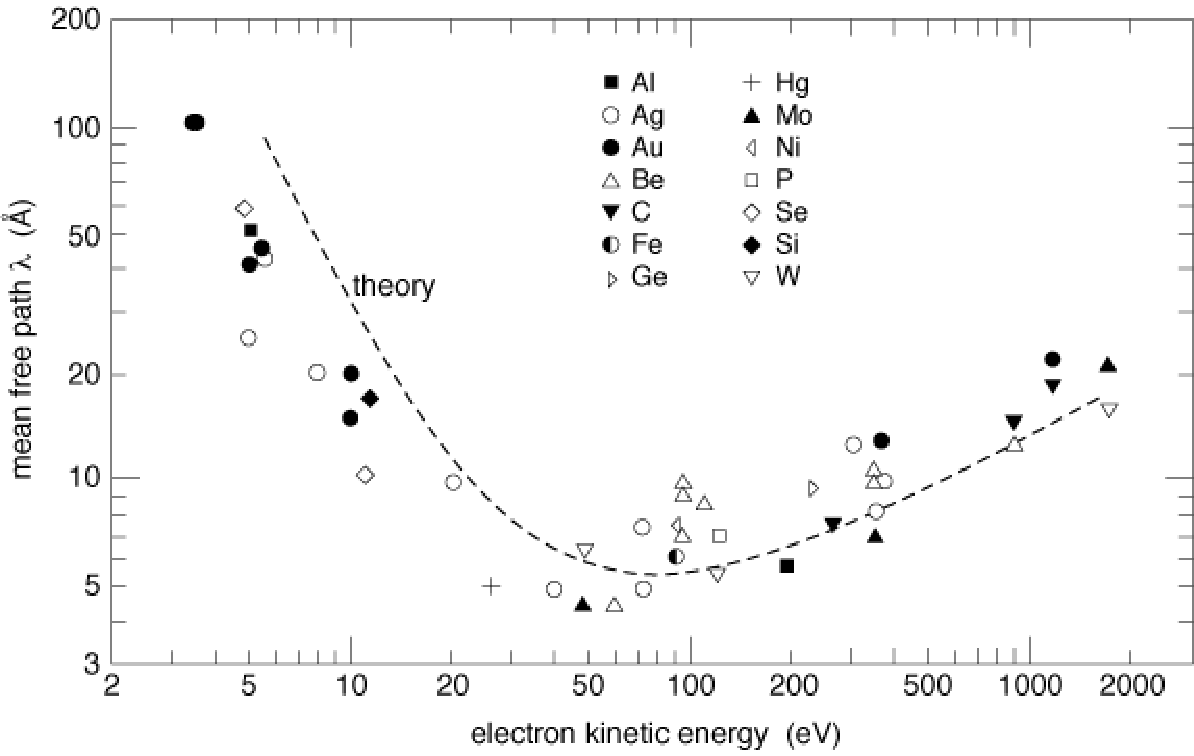
\includegraphics[width=\linewidth]{img/meanfree.pdf}
 \caption{\small Universal curve of solids \cite{zangwill}.  }
        \label{fig:uni}
\end{wrapfigure}


\FloatBarrier
\subsection{Energy Spectrum}
To understand the full spectrum of XPS it is necessary to understand each individual processes involved to be able to differentiate the peaks and draw any conclusion from their locations.


\subsubsection{Photoelectric Effect}
The most obvious contribution to the XPS spectrum is that of the photoelectric effect. A single electron absorbs the photon of energy $h\nu$, leaving the sample with a remaining energy of
\eq{E_\text{kin} = h\nu - E_\text{B} - \Phi \, ,}{}
where $E_\text{B}$ is the binding energy of this electron (relative to the Fermi energy) and $\Phi$ the work-function (minimum energy needed to remove an electron from a solid).
As there are only electrons in the atom up the the Fermi energy $E_\text{F}$, there are no electrons to be detected for (kinetic) energies greater than $h\nu -\Phi$. Typically this is used to define all measured energies relative to this Fermi energy.

This binding energy is not equal to the binding energy of the electron in a free atom. Bonds with the neighbouring atoms (chemical shift $\Delta E_\text{chem}$), electrostatic interaction with the whole lattice (Madelung constant $\Delta E_\text{Mad}$) and many-body effects of the hole in the final state (relaxation effects $\Delta E_\text{rel}$) influence the measured energy
\eq{E_\text{B}=E_\text{B,free} + \Delta E_\text{chem} + \Delta E_\text{Mad} + \Delta E_\text{rel} \; . }{}


\subsubsection{Auger Process}
When there is an electron missing in one of the inner shells of the atom, another electron from an higher shell will take its place. During this process either a photon will be emitted directly or the energy will be transferred to a third electron which now has enough energy to leave the atom. This latter process is called the Auger process. As XPS will remove electrons from the inner shells as well as the outer shells, this process will cause additional peaks in the spectrum. It is customary to label the Auger peaks with the shell-labels of the three electrons involved (eg. KLL for missing electron in the first shell, filling and leaving electron from the second shell). The positions of the Auger peaks are specific for the material being investigated.

The energy balance of the Auger-transition reads
\eq{E(KLL') = E(K) -E(L) - E^{*}(L') \; ,}{EKLL}
where $E(KLL')$ is the energy of the Auger electron stemming from a transition KLL', E(K)/E(L) are the binding energies of the electrons of the K/L-level and $E^*(L')$ is the binding energy of the electron in the $L'$ state, where the asterisk denotes, that this energy is altered through the absence of the $K$ and $L$ electron.

These formulas hold for free atoms. For an electron, that is emitted from the valence band of a solid the work-function has to be taken into account.


\subsubsection{Plasmons}
\label{sec:plasmonIntro}
The pseudo particle of fermi-gas oscillation is called a plasmon. These plasmons have characteristic energies, depending on the conduction electron density $n$. 
$$E_p = \hbar \underbrace{\sqrt{\frac{ne^2}{m_e \epsilon_0}}}_{\omega_p}$$
Eg. a calculation for aluminum, which has a conducting electron density of $n=1.8 \times 10^{29} \text{m}^{-3}$ yields $E_p(Al)=15.8 \text{eV}$.
Apart from the more obvious bulk plasmons (three dimensional oscillations in the sample) there are also surface plasmons when a material with positive dielectric constant (vacuum) interfaces with a material of negative dielectric constant (metal). Exact values for both bulk and surface plasmon energies for different materials are known in principle and can be looked up in the appropriate literature.

An electron that excites a plasmon looses one of these characteristic energies and is said to have suffered plasmon loss. It is possible, that one electron suffers plasmon loss several times, leading to a series of equally spaced losses with decreasing intensity.


\subsubsection{Shake-Up and Shake-Off}
%Impurities and lattice effects allow many-body interactions that would be impossible in a single atom. %??
Shake-up and shake-off events will divide the energy of the incoming photon between two electrons. Either one electron is emitted, leaving the atom in an exited state (shake-up) or both electrons are emitted (shake-off). Both effects depend on the energy levels of the atom and are thus characteristic for the material but are not as easily quantized as the other effect stated above.

Because the shake-off event can happen with even more than two electrons, it may lead to broad structures at the low kinetic (or high binding) energies of the spectrum.


\subsubsection{Satellite Peaks}
If the x-ray source is not monochromatic, there will be so called satellite peaks. The distance to the main peak and their intensity depends on the energy difference and relative intensities of the harmonics in the anode material of the x-ray source.



\section{Experimental Set-Up and Measurement Procedures}
\FloatBarrier
\subsection{Ultra High Vacuum (UHV)}
As the electrons that are detected easily interact with all kind of materials, it is very useful to operate in high vacuum. This is also necessary in order to reduce the rate of adsorption of molecules, which leads to disturbance of the measured spectra. (Ultra) high  vacuum (UHV) can only be achieved by a series of pumps acting within different pressure ranges.
\begin{wraptable}{r}{0.55\textwidth}
\begin{tabular}{lr}
\toprule
pump & pressure range (Pa)\\
\midrule
\small rotary vane pump & $10^5$ - $10^{-1}$  \\ 
\small turbo molecular pump &  $10^0$  - $10^{-9}$  \\
\small ion getter pump  & $ 10^{-3}$  - $10^{-9}$  \\
\small titan sublimation pump & $10^1$  - $10^{-9}$  \\
\bottomrule
\end{tabular}
\caption{Different pumps and their pressure operating range. \cite{gop} }
\label{tab:pump}
\end{wraptable}


\subsubsection{Rotary vane pump}
The rotary vane pump is a simple mechanical pump, which consists of a cylinder connecting the vacuum cell and the outer space. In the cylinder a vane rotates and thereby shovels the gas to the outside. Springs ensure optimal contact between the vane and the cylinder walls. 
\begin{figure} 
 \centering
\subfloat[][Rotary vane pump]
{        	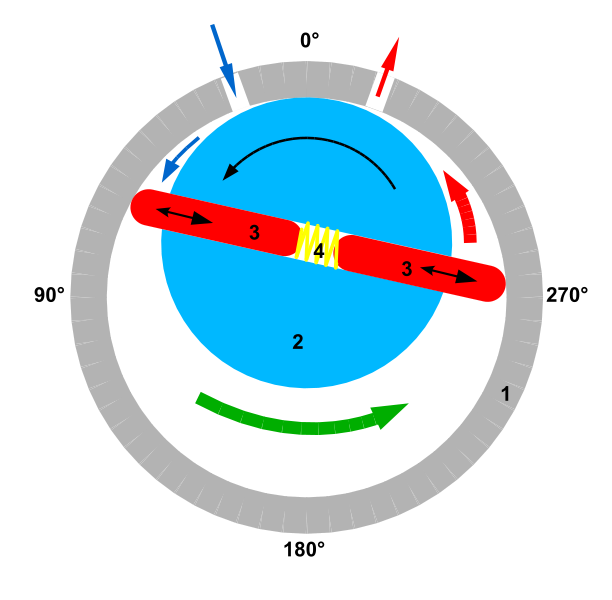
\includegraphics[width=0.45\textwidth]{img/rot.png}}
 \hfill
\subfloat[][Turbomolecular pump]
         { 	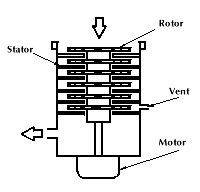
\includegraphics[width=0.45\textwidth]{img/tu.jpg}}
\caption{
\small \textbf{(a)} Rotary vane pump. 1: pump housing, 2: rotor, 3: vanes, 4: spring,  \textbf{(b)} Schematic description of a turbomolecular pump } 
	\label{fig:pump}
\end{figure}


\subsubsection{Turbomolecular pump}
The main features of a turbomolecular pump are the rotating blades (rotors), hitting the molecules very often per unit time, thereby enforcing a velocity distribution within the gas that is not isotropic, but a certain direction is preferred. Within the pump there are other static blades (stators), which act as a kind of filter to the velocity of the molecules in such a way, that molecules with the velocity, that is predominantly created by the rotors, can pass through with a higher probability. These filters act only in one-way, so that the molecules stay on the other side as long as the asymmetric velocity distribution is maintained. 


\subsubsection{Baking}
The above mentioned pumps can reach pressures of down to $10^{-9}\,\text{Pa}$ (cf. table \ref{tab:pump}). The remaining pressure, which is mainly due to the water molecules sticking to the walls of the chamber, can be lowered by thermal methods called baking. When the heated chamber with a pressure of still $10^{-9}\,\text{Pa}$ (due to the pumps still being active) is cooled down again, pressures of below $10^{-11}\,\text{Pa}$ can be reached. This process can take several days, so it is paramount to keep the pressure at this low level during and in between experiments.


\FloatBarrier
 \bibliographystyle{unsrt}
\bibliography{bib}

\end{document}


